\chapter{Introduction}

\section{Context}

In the last two decades, the blockchain technology \cite{Nakamoto:2008:RBP} has
emerged as a revolutionary approach to business \cite{noyen2014money,
  petukhina2020investing}, web services \cite{terzi2019blockchain} and
documentation of certain events, such as ownership transfers
\cite{wang2021nonfungible}. Many famous features and use cases of modern
blockchains highly rely on smart contracts \cite{khan2021}, first introduced at
2013 as one of the main features of Ethereum \cite{wood2014ethereum}. Smart
contracts allow performing a variety of actions related to cryptocurrencies in a
zero-trust manner making them a widely practised way of making anonymous
agreements, trading, and more.

The invention of smart contracts gave birth to a new programming paradigm. As
explained in the upcoming sections, decentralised applications have very
specific priorities regarding their implementations and take into consideration
issues that are usually not present in classical computer programs. One of their
most prominent value is having very defensive code, first aim of which is to
reduce the number of errors and unexpected behaviours as soon as it is possible.
While it is important to virtually all programs, smart contracts rely on it
exceptionally strongly, because they are impossible to be fixed after deployment
and the causalities of bugs in them can be frighteningly expensive.

In this document we present Hagia --- a liquid type refinement system that
supports verification of smart contracts written in the Sophia language
\cite{sophia}. Hagia has been written as an extension to the Sophia compiler and
its code is available on GitHub\footnote{Please refer to the related pull
  request at https://github.com/aeternity/aesophia/pull/334. The whole source
  code of the upgraded compiler can be previewed in the forked \texttt{aesophia}
  repository at https://github.com/radrow/aesophia/tree/hagia.}. This
dissertation focuses on its implementation and application for the smart
contract development, along with the theory behind it.

The following sections familiarise the reader with the idea of blockchain and
smart contracts --- first in a more popular context of the Ethereum network and
then moving to the case study of this work, which is the {\ae}ternity
blockchain. The next chapters introduce the Sophia language, discuss the need
for advanced type systems and present liquid types as a solution for the most
common issues of smart contracts. The \autoref{implementation} explains the main
algorithms and logics of Hagia and presents the source code of the most
important functions. The detailed implementations can be found in the linked
GitHub repository. At the end there is a presentation and discussion on how
Hagia enhances Sophia and what is its value for the ecosystem of {\ae}ternity.

\section{Blockchain}

Blockchain is a distributed data structure resembling a singly-linked list. The
main unit of a blockchain is a \emph{block}. Each block consists of a collection
of events called \emph{transactions} which most often represent virtual token
transfers and interactions with smart contracts. To keep the integrity of the
whole structure, every block stores the hash of the previous one making it
always clear which chain it belongs to and what its position is. Because of this
connection, changing, adding or removing any block in the middle requires
updating all following blocks as well, making forging chains virtually
impossible.

The participants of the network are usually called \emph{peers}, and those who
produce blocks are referred as \emph{miners}. Since miners are responsible for
keeping the blockchain alive, they are compensated for their work by being
credited with rewards in tokens and transaction fees of other peers. These fees
make denial-of-service attacks expensive and incentivise miners to validate
transactions and register them on the chain.

\begin{figure}[h]
  \caption{Blockchain visualisation}
  \centering
  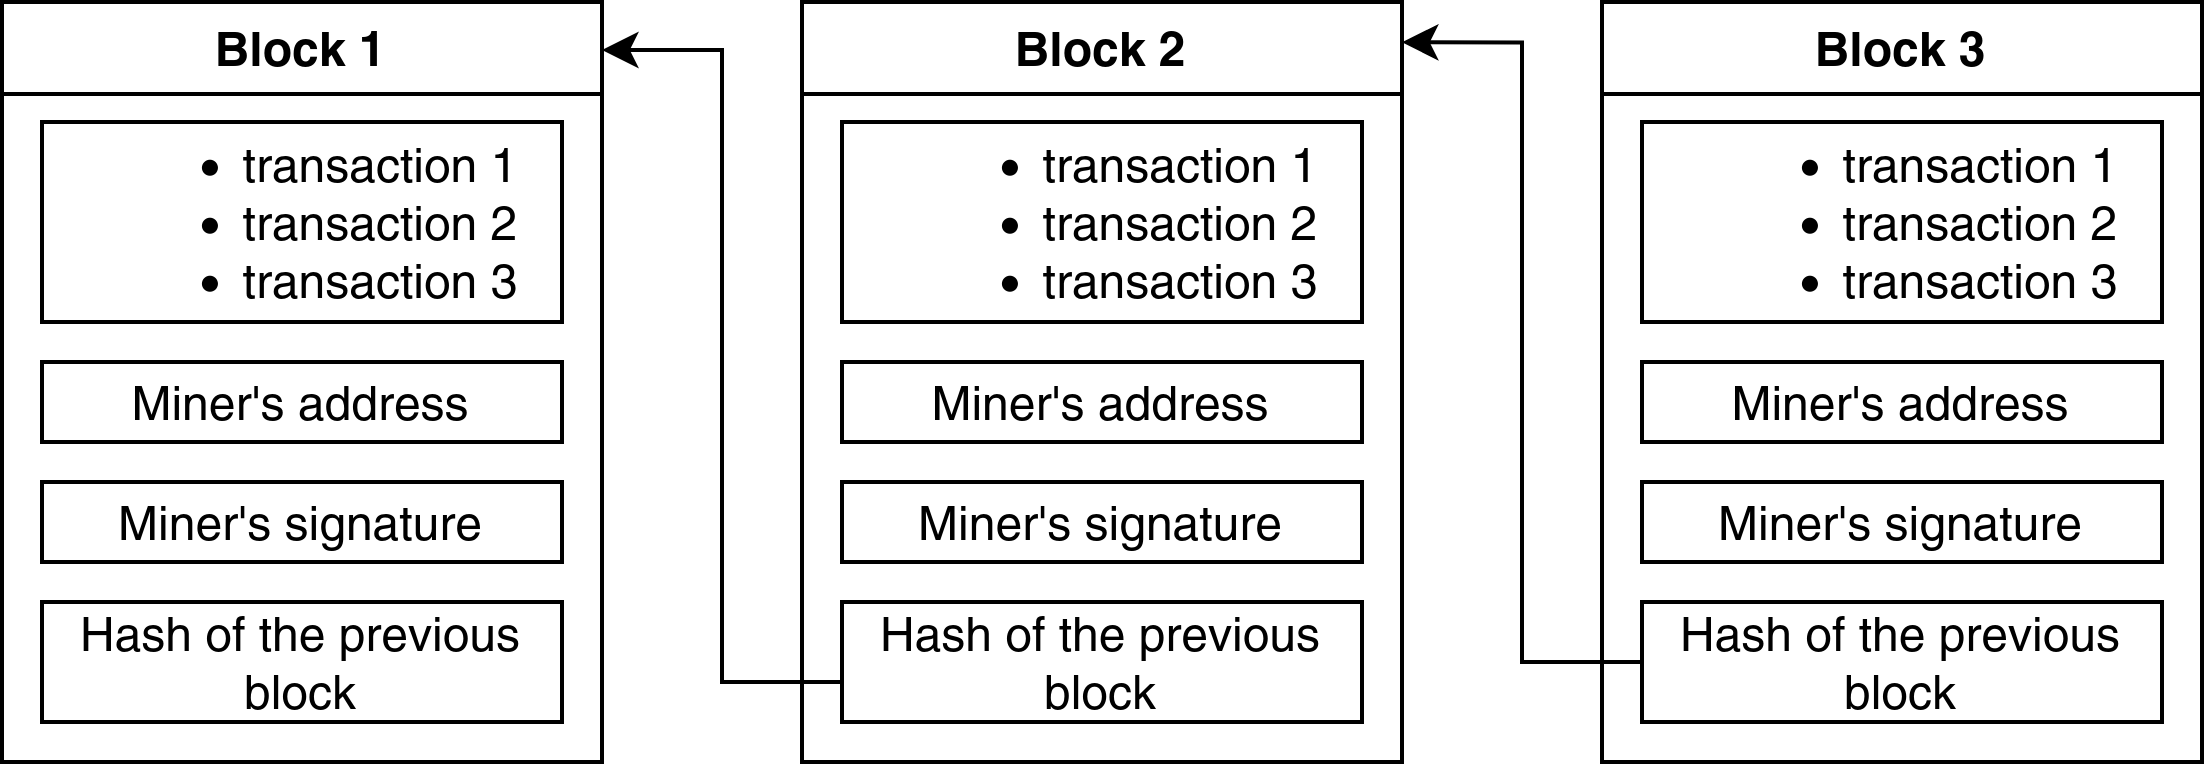
\includegraphics[scale=1]{blockchain}
\end{figure}

Each peer in the network is expected to keep at least some suffix of the chain,
so they do not need to rely on any centralised entity. Lack of a single point of
truth makes malicious peers, data races and hardware limitations a danger for
the integrity of the whole system, thus several algorithms to solve the problem
of synchronisation have been invented. The most popular ones are Proof of Work
(PoW) \cite{Nakamoto:2008:BPP} and Proof of Stake (PoS) \cite{King:2012:PPP}.
The former gains the security by forcing the peers to solve computationally hard
tasks, while the latter hands the right of producing new blocks to randomly
chosen peers based on the number of tokens they possess.

Such design aims to make the events on the chain immutable as soon as it is
possible. Owing to this, once a transaction has been placed on a blockchain, it
is nearly impossible to roll it back, because it would require convincing most
of the participants that the change is justified and shall not break any
assumptions. Consequently, no authority is able to undo an unwanted or misguided
action, assuming the network is properly secured.

\section{Smart contracts}

A smart contract is a computer program that acts as a first-class citizen in the
network. It owns tokens, may interact with other contracts, perform spend
transactions and accept incoming transfers. Due to the fact it lives entirely on
a blockchain, its behaviour is strictly defined by its immutable source code.

The most prominent smart contract language is Solidity, which compiles to the
Ethereum Virtual Machine (EVM). It is an imperative language highly influenced
by C and JavaScript, which supports some object-oriented programming features.
The EVM is a classical stack machine which additionally provides operations for
blockchain interaction.

Smart contracts allow making actual agreements between parties. As soon as all
the participants reach a consensus that the source code of a contract describes
the rules they want to follow, they can deploy it onto the chain and interact
with it. From this point on, the contract shall respond to their queries, manage
tokens and provide access to certain actions realising its purpose independently
and securely.

A basic example of such agreement would be a crowdfunding initiative: the
contract could accept and register incoming transfers and once the required
amount is reached, pay it out to the beneficiary. If the contract fails to
gather a certain amount up to a defined point in time\footnote{Time in the
  context of blockchains is usually measured in blocks which, in contrary to
  seconds, is not prone to synchronisation issues.}, it pays the tokens back to
the supporters. The investors do not need to worry if the rules are going to be
respected, as the power of the network secures it firmly.

One of the concerns arising from allowing computationally universal algorithms
to be executed on the chain is that not every peer might be able to evaluate
them entirely due to resource limitations. While there are some attempts to
statically put restrictions on the time and memory consumption, in general case
it is even impossible to tell if a given program ever returns \cite{turing1937}.
Owing to this, some additional mechanisms have to be introduced to eliminate the
risk of forcing peers to perform unrealistic computations.

One of the solutions involves so-called \emph{gas} as a remedy to that
problem \cite{wood2014ethereum}. Gas is a resource that must be acquired by the
caller before the contract is invoked. Each operation of the virtual machine
incurs a non-refundable gas cost. When the gas declared by the caller is
exhausted, execution stops and the transaction is reverted. The price of it and
the costs of particular instructions are adjusted so casual actions are
affordable, but performing heavier computations is costly.

The immutability of transactions gives a raise to a more problematic issue: if a
bug is spotted once the contract has been deployed, it cannot be fixed. The only
way to get rid of it is to create a new contract, migrate the state from the old
one and make all the parties aware of the issue\footnote{Of course, one must
  keep in mind that they do not have to agree on that and nothing stops them
  from abusing the contract.}. So far errors in smart contracts have made
significant harm to many entities exposing them to very damaging
loses \cite{peterjoost2018, olha.hlebiv2018, bishwascgupta2019, mattsuiche2017,
  christianreitwiessner2016}. Because of it, there is a great need for testing
and verifying contracts before they are let to the network.

\section{{\ae}ternity}

The case study of this research is the {\ae}ternity blockchain \cite{aeternity}.
At the time of writing it is a PoW chain implementing the BitcoinNG
\cite{Gencer:2017:SBT} protocol\footnote{As of September 2021 there are works on
  a custom protocol called hyperchains \cite{hyperchains}, which was first
  presented on 25th of August 2020}. It is highly inspired by Ethereum and
implements smart contracts, a naming system \cite{aens,
  brantlymillegannickjohnson2021}, oracles \cite{oracles} and state channels
\cite{state_channels, state_channels_eth}. One of the things that distinguish
{\ae}ternity from other chains is a custom smart contract programming language,
Sophia, which compiles to a proprietary virtual machine called Fast Aeternity
Transaction Engine (FATE) \cite{fate}. It shall be the main subject of analysis
in this work.

The project was established in 2017 by Yanislav Malahov and funded in an
ICO crowdfunding \cite{crunchbase2017}. The core code is written in Erlang with
some key parts implemented also in Elixir and Rust. It is entirely open source
and can be inspected in the official GitHub repository:
\url{https://github.com/aeternity}.
